\documentclass[a4paper]{article}   	

\usepackage[toc,page]{appendix}
\usepackage{graphicx}
\usepackage{subcaption}				
\usepackage{siunitx}
\usepackage{natbib}\citestyle{asa}
%\usepackage{mdframed}
\usepackage[a4paper,top=3.6cm,bottom=3.6cm,left=3.8cm,right=3.6cm,marginparwidth=2cm]{geometry}
\usepackage[section]{placeins} % keep figures in section
\usepackage{float}
%\usepackage{rotating}
\usepackage{amssymb}
\usepackage{amsmath}
%\usepackage{csvsimple}
\usepackage{pgfgantt}
\usepackage{textcomp}
\usepackage{bookmark}
\usepackage{hyperref}
\usepackage{titling} % Title page container
\usepackage{wrapfig} % Picture container


% flow chart
\usepackage[utf8]{inputenc}
\usepackage{tikz}
\usetikzlibrary{shapes,arrows, positioning}
% Define block styles
\tikzstyle{block} = [rectangle, draw, fill=gray!20, 
    text width=10em, text centered, rounded corners, minimum height=5em]
\tikzstyle{line} = [draw, -latex']
% for Chi-squared. Chi in line, not under line
\newenvironment{qhv}{\fontfamily{qhv}\selectfont}{\par}

\usepackage[automake]{glossaries}
\makeglossaries
\loadglsentries{glossary}

\setlength{\parindent}{0ex}
\graphicspath{{./figures/}}

% probably cancel calibration
\title{Remotely Sensed Resilience for the Prediction of Drought-Induced Forest Decline}
\date{\today}
\author{Sophie Christine Stuhler,\\sophie.stuhler@wur.nl}
			
%%%   Start Document   %%%
\begin{document}
\defcitealias{unepForest}{UNEP, 2010}
\pagenumbering{roman}
\setcounter{page}{0}

\begin{titlingpage} %Title Page, different setup, no page number
\thispagestyle{empty}
\newgeometry{top=1.25cm,bottom=0.96cm,inner=1.91cm,outer=1.91cm,foot=0cm,includeheadfoot} 
\begin{qhv}
	{\Large Geo-information Science and Remote Sensing}\vspace{0.7cm}
  
  {\Large Thesis Report GIRS-2018-53}\vspace{0.9cm}
  
  \hrule\vspace{1.1cm}
  \linespread{1}
  {\bfseries \Large \MakeUppercase{\thetitle}\par}\vspace{0.9cm}
  
  %{\bfseries \itshape (Subtitle)}\vspace{2.0cm}
  
  % Note: Remove the ``draft'' from \includegraphics to actually include an image, and adjust the vspace (padding) if you want to use a differently sized image
  \begin{wrapfigure}{r}{0.68\textwidth}
    \vspace{1cm}
    \includegraphics[height=12cm]{declineP10wins50bw4.png}
  \end{wrapfigure}
  
  {\Large \theauthor}\vspace{8.0cm}
  
  \rotatebox{90}{\Large \thedate}\vspace{1cm}
  
  % This is the vector version of the new WUR logo; due to layout changes it visually looks larger than the old one
  \sloppypar{\hspace{-2cm}\includegraphics[width=12cm]{title/WUR_RGB_standard}}
  
  % Note: this image is not stretched out like it is in the MS Word template
  \sloppypar{\noindent\makebox[\textwidth]{\hspace*{\dimexpr\evensidemargin-\oddsidemargin}\includegraphics[width=\paperwidth]{title/image2}}}
\end{qhv}
\end{titlingpage}

\newgeometry{top=3.6cm,bottom=3.6cm,left=3.8cm,right=3.6cm,marginparwidth=2cm} 
\thispagestyle{plain} % Subsequent page margins
\newpage\null

\newpage
\begin{titlepage} %Title Page, different setup, no page number

  % Note: this uses the MS Word template margins, you might want to increase them a bit for printing (e.g. inner=1.91cm,outer=1.91cm)
  %\thispagestyle{empty}
  \thispagestyle{plain} % Subsequent page margins
  \pagestyle{plain}
  \setcounter{page}{2}

  \begin{center}
  {\bfseries \Large \thetitle}\vspace{0.9cm}
  
  %{\bfseries \itshape Subtitle}\vspace{2.7cm}
  
  {\Large \theauthor}\vspace{0.9cm}
  
  {Registration number 92 04 30 815 070}\vspace{3.5cm}
  
  {\large \underline{Supervisors}:}\vspace{1.1cm}
  
  {Jan Verbesselt}\\
  {(Geo-Information Science \& Remote Sensing, WUR)}\vspace{0.5cm}
  
  {Arie Staal}\\
  {(Aquatic Ecology \& Water Quality Management, WUR)}\vspace{3.5cm}
  
  {A thesis submitted in partial fulfillment of the degree of Master of Science}
  
  {at Wageningen University and Research,}
  
  {The Netherlands.}\vspace{1.1cm}
  \end{center}
  
  \begin{flushright}
    {\thedate}
  
    {Wageningen, The Netherlands}
  \end{flushright}\vspace{0.5cm}

    Thesis code number: GRS-80436
  
    Thesis Report: GIRS-2018-53
  
    {Wageningen University and Research Centre}
  
    {Laboratory of Geo-Information Science and Remote Sensing}
    
\end{titlepage}    
\newpage\null\setcounter{page}{3}

\newpage
\section*{Abstract}
Although rates of tree mortality and forest decline are rising globally, there is still a lack of understanding the drivers and insufficient ability to reliably model the occurrence. Previous work has identified climatic factors and used a recent decline event in Catalonia to study the effect of soil moisture as seen from space and the effect of species. The research at hand identified Early Warning Signals as resilience indicators from vegetation indices of satellite time series to assess the stability of the forest ecosystems prior to this event on a large scale. Three different vegetation indices were used for the extraction of resilience indicators, each sensitive to a different type of plant functionality: NDVI to leaf chlorophyll content, NDMI to leaf water content and EVI to chlorophyll content and canopy structure. Strong trends of decreased resilience were found in areas with high forest decline occurrence. The resilience indicators were added to the existing logistic regression model and their significance, model fit and performance were reported. Overall, the best model explained about 31\% of the deviance in the data out of which an additional 4\% was explained by the resilience indicators. The most explanatory power within the Early Warning Signals was found in indices describing temporal autocorrelation when extracted from NDVI. However, the single best performing resilience indicator was the trend in spatial variance extracted from NDMI which explained about 1.3\% of the deviance in forest decline by itself.


\newpage
\section*{Acknowledgments}
This thesis has been an intriguing journey just like the entire master programme has been for me. It started with an environmental interest, observing with the persistent eyes of a satellite, analyzing in multiple dimensions with tools of Big Data, geostatistics, time series, and Machine Learning to create deeper understanding of the initial problem.\\
I am thankful for what I have learned, and the chances I was given, for the freedom and the critical and very supportive feedback, not only but especially during this thesis as well as throughout the past two years. I want to thank my supervisors Jan Verbesselt and Arie Staal for just the right amount of meetings to keep me questioning myself and their energy spent on following and guiding my thoughts and their enthusiasm for the topic. I have very much enjoyed your supervisison! I want to thank Jan Verbesselt, Ute Sass-Klaassen and Mathieu Decuyper for providing me with contacts and remarks during the development of the proposal. I want to thank Jordi Mart\'{i}nez-Vilalta, Mireia Banqué, Jordi Vayreda and David Chaparro at CREAF, Barcelona, for the reference data and their feedback on the results. I want to thank Dainius Maisili\=unas for advice on the technical questions of this research and Sytze de Bruin for feedback on statistics.\\
I am grateful to my parents and my sister Hannah for their financial and emotional support that made my studies possible in the first place. I want to thank Tim Jak and Robbert-Jan Joling for proof-reading, and finally I want to thank the thesis-room community for keeping the mood up at all times and the well-deserved Thursday-evening MGI 'borrels'.\\

\bigskip

Hartelijk dank!

\newpage % Table of Contents
\setcounter{page}{6}
\tableofcontents

\newpage
\listoffigures

\newpage
\listoftables

\newpage % Main Body
\pagenumbering{arabic}
\setcounter{page}{1}

\section{Introduction}\label{sec:intro}
Despite the urgency of the topic, our knowledge on causes and mechanisms as well as our ability to reliably predict tree mortality and forest decline on individual to regional scale are still lacking \citep{mcdowell2013, hartmann2015}. Forest ecosystems worldwide have been observed to show accelerating rates of tree mortality linked to drought stress and increased temperatures \citep{allen2010, chaparro2017, vanmantgen2009}. As climate change advances, this process is likely to intensify \citep{allen2015}, putting entire ecosystems at risk to undergo regime shifts. Tree mortality affecting a large part of a forest stand is known as forest decline \citep{martinez2012}. Forests globally are increasingly at the risk of declining \citep{choat2012} or in some areas even to undergo a regime shift, such as tropical forests transforming into savannas \citep{hirota2011}. This risk grows tangible in changes of frequency, intensity, duration and timing of fires and droughts, but also by the introduction of species, outbreaks of pests and pathogens, hurricanes, windstorms, ice storms, or landslides \citep{dale2001}. The phenomenon of tree mortality may occur at the level of the organism, but the processes leading to forest decline are observable and describable across spatial, organizational, and temporal scales and therefore demand for interdisciplinary approaches \citep{hartmann2015}.\\
A large study that synthesized findings on radial growth patterns prior to tree mortality found that the mortality is preceded by reduced growth rates in about 84\% of the cases \citep{cailleret2017}, and thus adding a temporal component and changes in plant productivity to the list of potential indicators of tree mortality. Temporal changes in forest responses to perturbations can also be characterized by remotely sensed \gls{resilience} \citep{verbesselt2016}. Remotely sensed \gls{resilience} makes use of the concept of Early Warning Signals \citep[EWS,][]{carpenter2006, carpenter2008, dakos2008}. These are indicators of resilience that are extracted from time series of satellite observations. These have the potential to reflect decreasing stability \citep{kefi2013} or even the approaching of a tipping point in the ecosystem \citep{scheffer2009b} based on slowing down observed through space and time.\\
So called Early Warning Signals (EWS) could provide the potential to warn in time when an ecosystem approaches a bifurcation \citep{dakos2014}. On the other hand, EWS can also be seen as a 'warning signal for a potential decrease in stability', independently of whether changes are catastrophic or not \citep{kefi2013}. Although EWS might not outperform direct (field) measurements of resilience \citep{vbelzen2017}, they still hold a big potential for predictive modeling especially for larger scales, remote areas and particularly for the modeling of past events. For the above described problem to explain drought-induced forest decline, they support the predictability as it is expected that a less resilient forest is more vulnerable to drought. Remotely sensed resilience could then contribute to large-scale predictions, and to the monitoring of forest decline risk and finally offer the possibility to look back in time \citep{verbesselt2016}. Since neither full understanding, nor methods to warn in time but as well as no accurate predictions of forest decline occurrence are available at this point, this research has great potential for forest management, as based on this, forest managers could adapt their planning. This research focuses on the predictive modeling of forest decline using both indicators of forest resilience and environmental variables that have proven to indicate part of the occurrence of forest decline \citep{chaparro2017}.\\
	

\newpage
\section{Problem Definition}\label{sec:problem}
According to the definition of the Food and Agriculture Organization of the United Nations (FAO), forest covers around 30\% of the earth's land surface \citepalias{unepForest} and their contribution to the terrestrial gross primary production of biomass is estimated at 75\% \citep{beer2010}. They take up atmospheric carbon and store it in their  biomass above and below the ground. But rising temperatures, changes in rainfall patterns and accelerating rates of climate change leave forests vulnerable to decline \citep{choat2012}. The physiological mechanisms behind forest decline are still not completely clear \citep{sala2010}, but also the explanation of the spatial occurrence is still pending \citep{chaparro2017}, so the question of 'what features are associated with forest decline?' is still not sufficiently answered.\\
Remote Sensing data offer the possibility to monitor on a large spatial and temporal scale. Using this asset, there have been studies on the impacts of tree mortality using remote sensing \citep[e.g.][]{breshears2005, meigs2011}, or analyzing extent and patterns after biotic-induced mortality events \citep[e.g.][]{meddens2012, wulder2006}. Remote sensing based resilience monitoring methods have demonstrated the potential to describe forest resilience on a large scale and its relationship with environmental factors \citep{keersmaecker2014, verbesselt2016}.\\
This thesis will look at the ability to predict forest decline with remotely sensed resilience indicators. This will be performed based on optical MODIS satellite imagery from which vegetation indices will be derived for the time span of the start of the MODIS mission in 2000, until the end of the growing season preceding a large drought-induced decline event that took place in Catalonia, northern Spain in 2012. From these time series generic temporal and spatial EWS will be derived and used as explanatory variables to model forest decline in the study area (Catalonia). The performance of the model will be tested independently. This approach will not focus on short-term external disturbances, such as windthrow, fire, or flooding, but will be seeking to reconstruct resilience in stress-induced forest ecosystems. Resilience indicators can be extracted because such dramatic events like forest decline are usually preceeded by changes in tree function as well as in structure \citep{hartmann2015}.\\
Since tree mortality is usually announced in reduction of growth rate and is thus a process that includes a temporal component, it is promising to assess the predictability from multitemporal data related to forest resilience, rather than trying to predict it from a snapshot (thus one single time step). This research therefore aims to predict forest decline on a grid-cell level of available satellite products using EWS as predictors from remote sensing time series. This thesis will assess the performance of remotely sensed resilience indicators (EWS) for the predictability of forest decline in a drought-stressed Mediterranean ecosystem.\\


\newpage
\section{Research Questions}\label{sec:rq}
The past decades have shown that the increasing frequency of drought events in Catalonia that puts forest ecosystems under stress which might result in more frequent forest decline events. Therefore, the overall goal of this research is to identify Early Warning Signals (EWS) from satellite imagery time series that can be used for predicting forest decline. The processes that lead to forest decline are still not clear. Previous research has shown the impact of climatic anomalies and soil moisture, but still failed to predict the spatial occurrence of such events. The EWS could potentially improve the predictability and be used to explain the role of resilience in the occurrence of forest decline. Three different vegetation indices (NDVI, NDMI, EVI) are used to extract resilience indicators from, each sensitive to different aspects of plant functionality and vitality. Therefore, the following research questions have been stated:

\begin{itemize}
\item Has there been Critical Slowing Down (CSD) prior to the forest decline event in Catalonia in 2012 which was captured in satellite time series?
\item If so, is the forest decline linked to the reduction in stability of the ecosystem?
\item Which EWS are most sensitive to explaining forest decline?
\end{itemize}

\bigskip
\bigskip


\begin{figure}[!h]
	\centering
	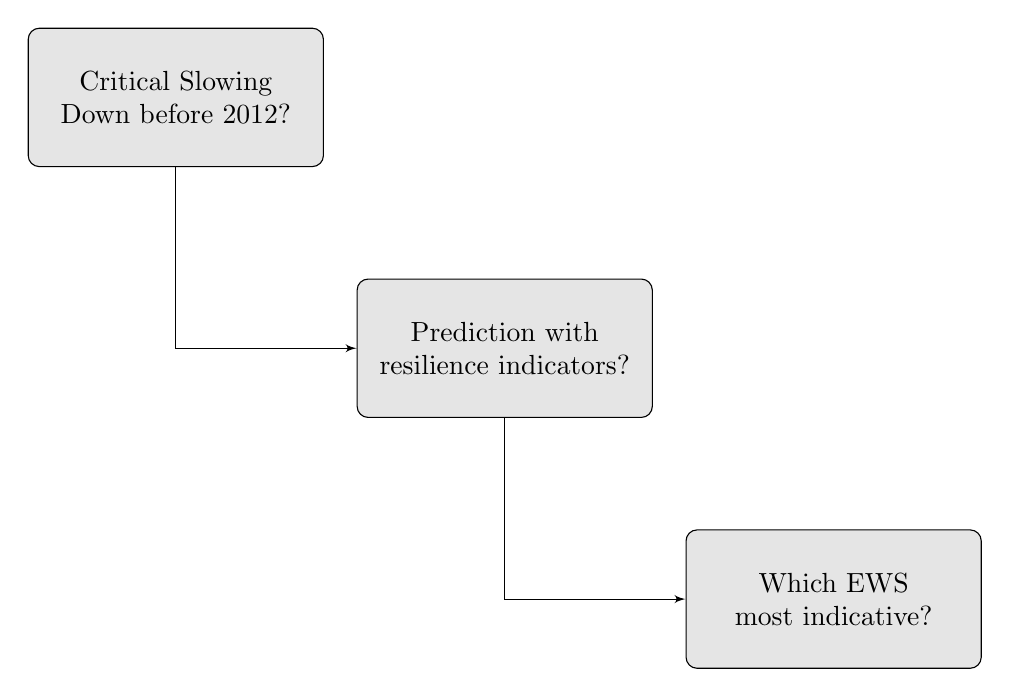
\begin{tikzpicture}[node distance = 2cm, auto]
		% node placement
		\node [block] (RQ1) {Critical Slowing Down before 2012?};
		\node [block, below right = of RQ1, xshift = -1cm] (RQ2) {Prediction with resilience indicators?};		
		\node [block, below right = of RQ2, xshift = -1cm] (RQ3) {Which EWS most indicative?};
		
		\path[line] (RQ1) |- (RQ2);
		\path[line] (RQ2) |- (RQ3);
	\end{tikzpicture}
\end{figure}





\newpage
\section{Theory on Tree Mortality, Forest Decline, and Early Warnings}\label{sec:theory}
Forest decline can be defined as tree mortality affecting an entire forest stand \citep{martinez2012}, but also leaf discoloration and leaf loss in a large extent can qualify as forest decline \citep{chaparro2017}. Either way, both definitions imply a large and obvious reaction of the forest indicating that a forest is massively affected. This thesis will focus on the latter where a forest is defined as declined if an area larger than 0.03~km\textsuperscript{2} shows tree mortality larger than 5\% or is affected by more larger than~50\% in the sum of both leaf loss and leaf discoloration in the canopies of at least one abundant tree species with a canopy cover larger than 15\% \citep{chaparro2017}.\\
Both the processes causing tree mortality and the exact definition of it remain a subject of research \citep{hartmann2015}. From a theoretical point of view tree death occurs at the point of minimum vitality \citep{dobbertin2005, grivcar2012}. From an anatomical and developmental perspective this point is less clear \citep{schenk2008}: one or more organs and tissues of the tree can for instance fatally desiccate when at the same time, other tissues like apical, cambial, and/or root meristems might still be intact and keep a plant alive.\\
The most commonly described physiological mechanisms causing a tree to die are hydraulic failure and carbon starvation \citep{sevanto2014}. Hydraulic failure describes this desiccation that might happen due to failed water transport \citep{mcdowell2011b}. Carbon starvation can be defined as the failure to maintain the metabolism or to defend against biotic agents when a negative carbohydrate balance is prolonged. These two mechanisms describing the plant vitality based on water transport and carbon assimilation, mobilization and concentration are expected to increasingly affect trees due to future extreme events \citep{brauning2017}. But also nutrient availability in the environment influences the survival of a tree since it affects the above-ground biomass allocation and can increase the water use efficiency and thus the risk of hydraulic failure and/or carbon starvation \citep{gessler2017}.\\
Tree mortality can be measured on different scales, e.g. by looking at the individual organism or at the plot level, where mortality is given as the percentage of dead trees. In this regard, a further differentiation based on species, angiosperms/gymnosperms is only applied in the form of accounting for species. Though, their coping mechanisms and thus their mortality rates against drought and stress differ  \citep[e.g.][]{chaparro2017}.\\
%especially on gymnosperms and drought induced mortality events (similar for drought together with biotic agents). but when biotic agents alone source of mortality: then shorter and more intense growth reduction (at p~\textless~0.1), with bark-beatle even more significant (p~\textless~0.05). longest and strongest growth reduction (median time for \(\Delta t_{m}~=~24~years\), annual growth ratio between dying and conspecific surviving trees at final stage, i.e. last year before mortality event \(g_{f,m}~=~0.29\)) found for other factors (not drought, not biotic agents; this includes interindividual competition)\\
%- species dying:\\
%like esh disease, directional, mortality only affecting specific species. can be observed from space, but due to spectral mixing and resolution mostly undetectable.\\
%from the ecological point of view very interesting, but restrained feasibility\\
The ability of a forest to remain in its initial state is called \gls{resistance} \citep[compare glossary for definitions, e.g.][]{keersmaecker2014}, which in this case means that the tree cover remains despite a distortion. That is, environmental factors may change, but the forest still does not suffer from it. Disturbance also might occur with an impact on the forest, but not causing it to shift into an alternative state, because it shows high \gls{resilience}. \Gls{resilience} is the return rate into the equilibrium state. In this case, individual trees might die, but the system will return to its initial state. \cite{dakos2014} describes resilience indicators from ecosystem time series. The idea is based on the fact that close to a \gls{tippoint} resilience is small. That is, a system with high resilience responds faster to perturbations, which is manifested as rising memory, variability and increased \gls{flickering}.\\
Natural ecosystems can shift from one stable state into another when a particularly heavy perturbation hits the system. This shift is called \gls{tippoint}. Other ecosystems have only one stable state and will recover from perturbations, or even reassemble without shifting to a qualitatively different state. That is, normally an ecosystem will tend to move back to a state of stability (\gls{basinattraction}) during environmental changes. If the system's resilience is low, it can be pushed over the boundaries and shift into an alternative stable state. Before this moment, the system exposes low resilience and a low recovery rate. With this the system's response to environmental impacts is more pronounced, which appears as increased variance and autocorrelation, which makes it observable in time series \citep{dakos2014}. Before the moment of transition, also called local bifurcation point, the recovery rate and \gls{resilience} span an angle of eigenvalue $\lambda = \ang{0}$. This results in apparent big impact of small disturbances, because the system needs more time to dissipate. This phenomenon is called Critical Slowing Down (CSD) \citep{dakos2014}. However, not all systems react in the same way when approaching a transition. Some regime shifts lack CSD completely. This is for example the case for strong abrupt changes in environmental conditions. But also less stable ecosystems that will not shift to another state can expose CSD.\\
\cite{dakos2012} implied two major challenges for detecting leading indicators: high-frequency sampling or experiments, and the lack of a clear framework. The former can be overcome with satellite data, as high frequency sampling is done by several satellites: the proposed MODIS NDVI data feature a revisit time of 1 day although not every observation can be used due to cloud coverage and other quality reducing factors. The clear framework of extracting leading resilience indicators is proposed in \cite{dakos2014}, who also launched a website for easy and low-threshold access at \url{http://www.early-warning-signals.org/home/}, where the framework, logical steps and theory is explained in simpler terms and with additional material.\\


\newpage
\section{Methods}\label{sec:methods}
%brief discussion of all the methods, why, how, ...


\subsection{Study Area}\label{subsec:studarea}
The Mediterranean is a vulnerable ecosystem that could be highly affected by climate change \citep{anav2011} with threats to the regional terrestrial carbon cycle and the vegetation dynamics. Climate change in the region is associated with higher temperatures, less rainfall and thus more drought and water stress for plants in the region. Catalonia was hit by several droughts in the past decades. 2004-2008, 2012 and 2016 were years with intense drought that affected large stands of the forested surface \citep{chaparro2017}. The forest decline of the drought-year 2012 was particularly intense in terms of forest decline occurrence. \cite{chaparro2017} already researched the environmental drivers of the declines, making it an ideal study area to assess the role of resilience in the occurrence of forest decline.\\
The study area included the entire forested surface of the region of Catalonia (Autonomous Community of Catalonia/Republic of Catalonia), which sums up to roughly 13000~km\textsuperscript{2} or 40\% of Catalonia's terrestrial surface \citep{chaparro2017}. Catalonia is widely forested and offers a variety of landscapes and climates due to the presence of the Pyrenees in the North and the proximity to the Mediterranean Sea in the Southeast and the Central Depressions and coastal mountain ranges. Climatically it is classified into Alpine climate in the Pyrenees, Maritime or Oceanic in the valleys and Mediterranean on the coast and the inland. It is thus diverse and features different kinds of climatic and environmental conditions for the vegetation. It features not only large areas of forest at the boundary of two biogeographic regions (Mediterranean and Euro-Siberian) but also a variety in climatic variables such as mean annual rainfall and temperature, as well as their annual distribution, but also different species. The most frequent tree species are \textit{Pinus halepensis} covering 2430~km\textsuperscript{2} and \textit{Quercus ilex} with 2000~km\textsuperscript{2} \citep[\citeauthor{chaparro2017}, \citeyear{chaparro2017} after][]{creafsol}.\\
The DEBOSCAT network in Catalonia is a unique survey for the assessment of forest health with field data describing all forested areas $>$ 0.03~km\textsuperscript{2} that were affected by forest decline. Small forest patches affected by forest decline were not included in the analysis, that is False Negatives of less than 0.03~km\textsuperscript{2} might occur and bias the result as they might indeed show CSD. Although droughts are common in the region, the 2012 drought was characterized by intense temperature anomalies affecting broadleaved species in particular \citep{chaparro2017}. It was preceded by a drought that lasted from October 2004 until October 2008, which might have already weakened the abundant forests and lowered their resilience. Most of the declined forests are situated inland. A cluster with many declined plots shows up northeast of Vic, a smaller one around Solsona and some more around the Central Depression. For a detailed map of the declined plots see figure \ref{studarea}.


\begin{figure}[H]
	\centering
	\makebox[\textwidth][c]{\includegraphics[trim = 0 20 0 10, clip, width = 1.2\textwidth]{DeclineMask2012.png}}
	\caption{Overview of the forest extent in Catalonia, declined forests are marked as grey polygons.}\label{studarea}
\end{figure}



\subsection{Data}\label{subsec:data}

\subsubsection{Sensors}
By now, there is a variety of optical sensors in space with differing spatial and temporal resolution that fit the purpose of vegetation monitoring. Common pixel sizes vary between 1.5~m (e.g. SPOT Végétation) and several hundreds to thousands of meters (e.g. MODIS, MERIS, Sentinel-5 Tropomi). The revisit time of these sensors mostly depends on the number of satellites supporting the fleet and the footprint per sensor. Recently launched Sentinel-2 operates with two identical satellites to provide a temporal resolution of 5 days at the equator and 2-3 days at mid-latitudes. For the study at hand, not only spatial resolution, but also temporal resolution and the length of the archive matter, since the number of data points (time steps) for each time series should still be given with a high revisit time to ensure sufficient cloud-free observations and long archive. Recent work showed that the spatial resolution was less important than the temporal when extracting EWS (Hendrix, in preparation).\\
Therefore, the mid-resolution MODIS optical sensor was chosen, since it provides global observations in 1-day intervals due to its wide swath width \citep{modisvcf}. This revisit time allows for a dense time series. Covering such a large area comes at the cost of ground resolution (250~m). The MODIS mission operates on two satellites, Terra and Aqua, which were launched in 1999 and 2002, respectively, and which are both still operating. Their main difference is the orbit in which they fly. Terra's main goal is earth observation for land products, Aqua in contrast aims at sea products. To capture the land surface mostly cloud-free Terra's local orbiting time is 10:30~a.m. in descending mode, Aqua around 1:30~p.m. in ascending mode.\\
Optical sensors refer to camera-like sensors. The technique describes the capturing of a range of wavelength in the electromagnetic spectrum (i.e. a band), therefore also called multispectral (multiple spectra). This wavelength range can represent the visible light, near-infrared (NIR) or short-wave infrared (SWIR). Since the light source is mostly the sun, these are called passive instruments: they only capture energy, but do not emit any (in contrast to active radar instruments).\\
The amount of reflected energy depends on the albedo of a surface and is unique to each surface. Hence is it theoretically possible to classify and characterize each surface based on its reflectivity.
The processes of transmission, reflection, and absorption already feature the importance of knowing the amount of energy emitted by the sun as well as the given processes in the atmosphere to remodel the according reflectance of a given pixel. Therefore, optical remote sensing data can be classified into different processing levels. The dataset used in this thesis was processed or accessed to Level~3 (ready-to-use products: including georeference).\\


\subsubsection{Indices}
The vegetation indices aimed to depict different ground processes that were expected to exhibit CSD. These processes are a representation of plant vitality and/or leaf properties. The first index is called Normalized Difference Vegetation Index (NDVI). NDVI is mostly sensitive to photosynthetic activity. That is because chlorophyll-a and chlorophyll-b absorb light in the red and green spectrum, but highly reflect in NIR. Typical vegetation spectra with varying chlorophyll contents can be seen in figure \ref{fig:vegspec}.

\begin{figure}[htp]
	\centering
	\begin{subfigure}{0.49\textwidth}	
		\centering
		\includegraphics[width = 0.95\textwidth]{veg_spectra_CAB}
	\end{subfigure}
	\begin{subfigure}{0.49\textwidth}	
		\centering
		\includegraphics[width = 0.95\textwidth]{veg_spectra_CW}
	\end{subfigure}
	\caption{Typical vegetation spectra with LAI = 4, varying chlorophyll and leaf water content modelled in SLC demo \citep{verhoef2007}. Higher chlorophyll content lowers the reflectance in the visible light, whereas leaf water content influences the absorption of light in higher wavelengths.}\label{fig:vegspec}
\end{figure}	

NDVI was calculated by dividing the difference of the reflectance of these bands over their sum \citep[\textit{cf.} formula \ref{eq:ndvi}, after][]{tucker1979}. High photosynthetic activity is thus shown with a high NDVI. NDVI is widely known and widely used due to its easy calculation and relative robustness against varying atmospheric conditions.\\
% NDVI literature
% NDVI formula
\begin{equation}\label{eq:ndvi}
	NDVI = \frac{R\textsubscript{NIR} - R\textsubscript{Red}}{R\textsubscript{NIR} + R\textsubscript{Red}} 
\end{equation}\\

The Enhanced Vegetation Index (EVI) works similar as the NDVI, but accounts for high LAI-values. NDVI tends to saturate at high LAI values. By applying a gain factor to the entire fraction and accounting for canopy as well as aerosol background conditions, it overcomes this obstacle and is more sensitive to LAI and canopy architecture \citep{liu1995}. It was calculated as follows:\\
\begin{equation}\label{eq:evi}
	EVI = 2.5 \times \frac{R\textsubscript{NIR} - R\textsubscript{Red}}{R\textsubscript{NIR} + 6 \times R\textsubscript{Red} - 7.5 \times R\textsubscript{Blue} + 1}
\end{equation}\\

NDMI compares the NIR with the SWIR water absorption feature at 2.1~-~2.3~\textmu m \citep[\textit{cf.} formula \ref{eq:nbr}, after][]{garcia1991}. The NIR reflectance is mainly influenced by the LAI (leaf area index), looking angle and the distribution of the light according to the bidirectional reflectance distribution function (BRDF). Photosynthetically active vegetation shows characteristic behavior in this wavelength region with very high reflectance compared to other surface types. It can reach up to 70\% reflectance in planophile plants with high LAI. The water absorption feature in the SWIR reflectance is mainly influenced by leaf water content (\textit{cf.} fig. \ref{fig:vegspec}), but also LAI. Originally, the NDMI was developed to show fire scars in vegetation (as Normalized Burnt Ratio), but since it is sensitive to changes in leaf water content, it could possibly depict CSD in water availability in the leaves - particularly in the canopy - and water transport, too.\\

\begin{equation}\label{eq:nbr}
	NDMI = \frac{R\textsubscript{NIR} - R\textsubscript{SWIR}}{R\textsubscript{NIR} + R\textsubscript{SWIR}} 
\end{equation}\\

The time series were derived from the MOD13Q1.006 Terra Vegetation Indices 16-day Global composite at 250~m resolution \citep{modisvcf}. This is a Level~3-product retrieved from the daily observations of MODIS Terra. These get corrected for atmospherical influences. The 16-day value is the pixel value selected by an algorithm that chooses the closest-to-nadir pixel from the two highest NDVI-observations. It works successfully in all ecosystems, so no constraints were met for the use of this product. The vegetation indices product only features NDVI and EVI, but is provided with the necessary NIR and SWIR bands, so NDMI could be calculated as well. NDMI was calculated after the initiation phase of the SWIR sensor, that showed malfunctioning in its first year of operation (2000-2001).\\

%\subsubsection{Radar Data}\label{subsubsec:radar}
%Radar instruments capture energy in the microwave spectrum. Usually spaceborne radars are active instruments with a side-looking antenna. It emits polarized microwaves and detects the amplitude and phase of the backscattered wave. This allows for substantially different analyses than optical instruments. As a rule of thumb, electromagnetic waves interact with objects and structures of size of at least their own wavelength. As such, microwaves transmit the atmosphere for their biggest part, not like optical data that is highly influenced by cloud coverage.\\
%Secondly, since the phase of the wave can be measured, this technology allows for analysis of polarization. This comes in handy for vegetation monitoring. Vegetation is the main source of depolarization. As the microwave hits, for instance, a forest the wave will partially penetrate and interact with either branches or the trunk - depending on the wavelength (frequency). Due to depolarization and socalled volume-scattering microwaves are sensitive to biomass(literature).\\
%
%
%% proper placement of the below paragraph
%The above described data sources and different indices are all sensitive to different leaf properties: NDVI and EVI are sensitive to chlorophyll content and thus to photosynthetic activity, NBR to leaf water content, and VOD mostly to biomass. Therefore, they cover a wide range of parameters where CSD can be expected. The main difference between NDVI and EVI is that NDVI saturates at high LAI-values. However, it is very easy to calculate and widly used and known. I would expect EVI to be more sensitive to CSD, but the user community might be more susceptible to implement NDVI-based EWS since familiarity is given.
	

%\subsubsection{Dendrochronology Database}\label{subsubsec:dendrodb}

%a) MODIS NDVI, LAI, EVI, NBR? AMSR-E VOD? MODIS on Terra \& Aqua satellites: time series of NDVI multispectral data since 1999 offers long-term time series with medium resolution (200~m) for earth surface monitoring\\
%b) Landsat NDVI, EVI, since 1972\\
%Level 3, products. explanation of pre-processing and product generation\\
%optical/multispectral data, radar data\\



\newgeometry{top=2cm,bottom=2cm,left=2.7cm,right=2.7cm,marginparwidth=2cm}

\begin{figure}[htp]
	\centering
	\includegraphics[width = 0.98\textwidth]{FlowChart_MSc_thesis}
	\caption{A schematic framework of analysis performed in this research including preprocessing, predictor extraction, prediction, validation, and indications for each research question.}\label{fig:flowchart}
\end{figure}	

\restoregeometry{}

\subsection{Data Analysis}\label{subsec:analysis}
A schematic framework belonging to the steps followed in the analysis can be found in figure \ref{fig:flowchart}. The overall idea follows the scheme of preprocessing of the satellite images into regular pixel time series, predictor extraction from the time series in the form of Early Warning Signals (EWS), setting up a null model based on previous research, setting up several extended models with the extracted EWS and finally comparing their performance against the null model on a test dataset.\\



\subsubsection{Preprocessing}
Preprocessing included the removal of pixels with low quality flags (QA~VI~$>$~1), filtering by date, clipping to the study area, NDMI calculation, outlier removal, and NA-interpolation. Quality flag values of VI~$>$~1 refer to pixels that are affected by the presence of clouds, haze, shadow, snow or high aerosol content. For capturing the resilience of the forests prior to the forest declines, the time series were cut off at the end of 2011 to not obtain a biased resilience-estimate. To obtain the time series for the study area the time series were clipped roughly with a hand-drawn polygon within Google Earth Engine and later on clipped to the the boundaries of Catalonia using the database of Global Administrative Areas \citep[GADM, see][]{gadm}.\\
The MODIS vegetation indices product \citep[VCF,][]{modisvcf} is a product already aggregated to regular time series of 16-day intervals (equidistant time series) so no further aggregation was needed. The product features time series of NDMI, EVI, surface reflectance values of the blue, red, NIR, and SWIR band and several other metadata band. The calculation of NDMI values was therefore performed per pixel using the NIR and SWIR bands of the VCF product.\\
Outliers were identified from a given pixel time series if they were outside the H-spread range \textit{H} given by the inter-quartile range multiplied by a mildness factor of 1.5 (compare equation \ref{eq:outliers}). The interpolation of missing values was done by linear interpolation when values were detected outside the interval of 1.5 times the interquartile range(IQR) of a given time series. If missing values were present at the beginning or end of the time series, the first/last value was replicated to avoid extrapolation.

\begin{equation}\label{eq:outliers}
\begin{aligned}
	H = 1.5 \times IQR\\
	IQR = Q3 - Q1
\end{aligned}
\end{equation}\\


The null model used in this analysis is based on 1~km products \citep{chaparro2017}, so the predictors extracted from the MODIS time series needed to be resampled to this resolution. This was done by bilinear interpolation: averaging the values of the surrounding cells \citep{bernstein1976}. This form of upscaling made sure, that the given plots matched the time series at hand. That is, location, mask and extent of the measured plots were represented by the according pixels from the remote sensing data. The used MODIS pixels spanned an area of 250~m~$\times$~250~m on the ground \citep{modisvcf}. To assure that only forested pixels would be analyzed, pixels with a tree canopy cover of less than 10\% (based on the MODIS VCF product) were masked out, according to the FAO's definition of forest \citep{faoforest}. The FAO defines forest as "land with $\geq$10\% tree canopy cover that is not used for agriculture or settlement, or has~$<$10\% tree canopy cover but is regenerating" \citep{bastin2017}. Tree canopy cover between 10\% and 39\% classify as open forest and above 40\% as closed forest. Visual inspection of the tree canopy cover in the study area showed that low values referring to open forest are encountered frequently, as was expected for dry European forests \citep{bastin2017}. So the satellite time series were masked with pixels of open forest, hence a threshold of 10\%.



\subsubsection{Predictor Extraction}
For describing the occurrence of forest declines, a set of explanatory variables was extended with Early Warning Signals (EWS) to investigate whether they can be used to improve the predictability. These EWS are all based on the theory of Critical Slowing Down (CSD) as an indicator of an approaching \gls{tippoint}, that can be seen as leading indicators of \gls{resilience}. An ecosystem with high \gls{resilience} should show lower values and a weaker trend in the metrics than a less resilient ecosystem in which indicators are expected to rise \citep{scheffer2001, scheffer2009a, carpenter2011a, dakos2012, dakos2014}.\\
In the following, the steps required for the extraction will be laid out.\\

\paragraph{Detrending:}
Detrending aimed at the removal of trends in the time series that might recur, but have no influence on the rise of e.g. variability or \gls{flickering} \citep{dakos2012}. If the trends are not properly removed the EWS might follow the pattern of the trend. An example for desired detrending is removing seasonality. Detrending of the time series needs to be carried out carefully, as with higher order trend-differencing we might easily overfit the data \citep{dakos2008} and thus remove exactly those deviations from the equilibrium that are actually of interest, since they result from the perturbations and disturbances from which the EWS are calculated. As described above, the main trend in the data followed the pattern of seasonality. A Gaussian kernel function was applied over the time series since it showed to be very flexible. The bandwidth of the Gaussian kernel was assessed in a separate sensitivity analysis.\\

\paragraph{Window Size:}
Typically, the window size is half the length of the time series \citep{dakos2012}. But in case of fast timescales of a system, a shorter window length is needed (analogously for longer time scales). Still, smaller time scales result in less accurate estimate of the metric at use. Therefore, different window sizes were tested in the sensitivity analysis for the leading indicator autocorrelation. Autocorrelation is sensitive to the choice of window size and was used to assess whether the typical value of half the length of the time series approximates an appropriate response time.\\

\paragraph{Sensitivity Analysis:}
Due to the various possible choices of parameter settings, the selection of parameters for the extraction of the EWS needed special attention. The parameters that influence the outcome are (as mentioned above) mainly the choice of detrending and the size of the rolling window. The usual procedure for assessing the sensitivity of an EWS to a parameter is by visualizing the outcome for a range of values \citep{dakos2008}. The difficulty of this thesis compared to \cite{dakos2008} is to find an optimal parameter setting for a dataset consisting of several thousand different time series (one per pixel) and different climatic zones. To automatically detect and assess an optimal parameter setting for each time series was considered outside the scope of this thesis. However, the idea of visually assessing the sensitivity analysis of the parameter setting was preserved. 30~pixels were randomly chosen in a stratified random sampling (affected/not affected by forest decline served as strata) for which the sensitivity analysis was carried out (the spatial distribution of the randomly selected points within the study area can be seen in figure \ref{studarea}). Heatmaps of both the trend statistic for ACF-1 (temporal autocorrelation at lag-1) and its according significance were visually analyzed to compare the sensivitity of the trend on changes in either one of these parameters: rolling-window size against the bandwidth of the Gaussian kernel used in detrending. The analysis was further conducted by visually assessing the detrended time series at the same time to confirm successful detrending. Eventually, the parameter setting that showed the strongest significant trend in most analyzed points was chosen.\\



\paragraph{Generic metric-based EWS:}
Although there is a wide variety of EWS, they can be grouped based on which CSD phenomenon they describe: rising memory, rising variability and \gls{flickering}. As flickering between dead and alive forests was not expected, the focus lay on the easier to calculate generic indicators describing either rising memory or rising variability: ACF-1, AR(1), standard deviation, skewness, kurtosis and density ratio. They all belong to the group of generic metric-based indicators. In contrast, model-based indicators fit a specific model-type.\\
The EWS at use will be described in the following section:\\
\begin{itemize}
	\item Autocorrelation (ACF(1)) and Spectral Properties. Autocorrelation at lag-1 (AR(1)) is the most basic indicator of CSD. It determines the correlation between a data point \textit{n} and its neighboring point \textit{n~-~1} \citep{carpenter2008}. Different metrics are proposed, all referring to the auto-regressive (AR) coefficient which is mathematically similar to the autocorrelation function. These metrics are therefore describing similar patterns of rising memory. Namely those are the auto-regressive coefficient of the AR(1) model \citep{held2004} and the return rate \citep[inverse of AR(1) model][]{carpenter2008}. Further similar metrics, that account for correlation in higher lags are subsumed under the term spectral properties. That is, rising memory will be observed in so called spectral reddening. They derive the EWS from the power spectrum. EWS are spectral density \citep{kleinen2003}, spectral exponent \citep{dakos2012}, and spectral ratio of low to high frequencies \citep{biggs2009}.
	\item Variance by Standard Deviation (StDev). Based on the observation that close to a transition slowing down, \gls{flickering} or both can be observed. Both of these phenomena can be captured by StDev and the CV. They both describe the fluctuation around the mean, that is they quantify the deviation from the stable state \citep{carpenter2006}.
	\item Skewness and Kurtosis. Close to a transition, we observe slow dynamics \citep{scheffer2009b}. Because skewness measures the symmetry of a dataset, slow dynamics will result in a left- or right-skewed distribution \citep{guttal2008}. It is defined as the third moment around the distribution's mean. Depending on whether the alternative state is larger or smaller than the present one, skewness will become positive or negative \citep{dakos2012}. Kurtosis describes the deviation from normal distribution in \textit{y}-direction. In other words it describes whether the slopes of the peak of a distribution are steeper or less steep than the ones of a normal distribution and is hence mathematically defined as the fourth moment around the distribution's mean. In case of a transition we expect the tails of the time series to become fatter \citep{biggs2009}, that is the distribution becomes leptokurtic because rare values will occur more frequently \citep{dakos2012}.
\end{itemize}

\paragraph{Spatial EWS:}
Many environmental processes exhibit spatial patterns. Spatial Early Warning Signals are based on the assumption that systems become increasingly spatially homogeneous at close distance when approaching a critical transition, and thus more spatially correlated \citep{kefi2014}. The choice of the spatial EWS depends on the presence or absence of specific spatial patterns, their derivation is otherwise senseless if changes in a certain pattern are absent there will also be no change among them. Among these, patterns like periodicity, anisotropy, and patchiness need to be evaluated for the case at hand. Periodicity will be removed through detrending. Anisotropy refers to a directional spatial gradient. Patchiness is given if the forest consists of e.g. shrubby patches and open patches. Neither did the forests show multiple stable states, nor periodicity in the time series (after detrending) nor patchiness, so the spatial EWS only included the temporal trend in spatial autocorrelation, spatial variance and spatial skewness as well. These are calculated on the pixel distribution within a given spatial distance \citep{kefi2014}, thus within a moving window of 3~$\times$~3 pixels. These three spatial indicators were calculated at each time step and used as input to the trend quantification (see next paragraph).\\
\begin{itemize}
	\item Spatial Correlation at Lag-1. Local Moran's I is a Local Indicator of Spatial Association \citep[LISA,][]{anselin1995}. It was calculated as the deviation of the mean of the neighbouring cells compared to that of the center cell \textit{i}:
	\begin{equation}
		I_i = z_i \sum_j w_{ij}z_j
	\end{equation}
	where $z_i$ and $z_j$ are the deviations from the mean and $w_{ij}$ are weights given in a weights matrix. The weights matrix used in this thesis assigns a value of 1 to all 8 neighboring cells, also called Queen's case.
	\item Spatial Variance. Spatial variance was calculated as the variance within a kernel of 3~$\times$~3 pixels.
	\item Spatial Skewness. Similar to spatial variance, spatial skewness was derived as the skewness of values within a 3~$\times$~3 kernel.
\end{itemize}




\paragraph{Trend Quantification:}
Kendall's $\tau$ rank correlation coefficient \citep[after][]{kendall1938} was used for testing against the null hypothesis of randomness of the measurements against time \citep{dakos2012}. The value of $\tau$ increases in case of a positive trend over time. That is, the respective EWS increases over time. Analogously, it decreases in case of a negative trend. In case of the null hypothesis of randomness in the trend, Kendall's $\tau$ is expected to show low absolute values. Spearman's $\rho$ rank correlation or Pearson's correlation coefficient would both also be valid trend measures. However, for time series analyses and EWS Kendall's $\tau$ is most frequently used, so it was also the statistic of choice for this analysis. If the time series (of the EWS) is free of ties with the time vector (converging with time), Kendall's $\tau$ was calculated as given in equation~\ref{eq:kendall}. In case of ties the algorithm \citep{mcleod2005} performed a continuity correction as described in \cite{kendall1976}. 
\begin{equation}\label{eq:kendall}
	\tau = S / D \\
\end{equation}	
where 
\begin{equation*}
\begin{aligned}
	S = \sum_{i < j} (sign(x[j & ] - x[i]) \times sign(y[j] - y[i])) \\
	&D = n(n - 1)/2
\end{aligned}
\end{equation*}\\

\subsubsection{Principal Component Analysis}
The response variable forest decline is binary and qualitative (declined~=~1, not affected by decline~=~0). This was modeled based on the logistic regression model by \cite{chaparro2017}. Logistic regression means that the underlying mechanisms are linear in a way that the log-transformed odds follow a linear relationship with the predictors. This holds advantages as the interpretation is more straight-forward: an increase in a given predictor leads to a higher or lower probability of an observation being classified as a success (see chapter below on the prediction). But on the other hand correlation between predictors leads to an incorrect estimation of the explained variability and relationship. This problem is called multicollinearity and its magnitude can be estimated by the Variance-Inflation Factor (VIF).\\
The EWS all indicate resilience, making them per se correlated. To overcome the correlation, the predictor set of the trends of the EWS was transformed with a Principal Component Analysis (PCA). The PCA decorrelates a given feature space by rotating it towards the axes of maximum variance \citep{james2013}. Each axis is constructed orthogonal to all others. The rotation axis is defined as the loading vectors $\phi_1 , ..., \phi_p$ for each Principal Component (compare equation \ref{eq:loadvectPCA} for the first PC Z\textsubscript{1}): 

\begin{equation}\label{eq:loadvectPCA}
	Z_1 = \phi_{11}X_1 + \phi_{21}X_2 + ... \phi_{p1}X_p
\end{equation}\\

The decorrelated first Principal Components explaining up to 95\% of the cumulated variability in the EWS-trend dataset were then used in the prediction to extend the null model. As PCA rotates the feature space towards the highest variability, a so called elbow effect will take place. This means that most information in the dataset can be contained in the first Principal Components. These are characterized by high explained variance and high eigenvalues. Both the explained variance and eigenvalue will show a flattening effect (elbow). Therefore, only the subset of first Principal Components explaining this majority of information will be used in the prediction. To understand why a certain Principal Component shows significance, the magnitude of relationship of each EWS-trend with their according loading vectors were inspected.\\


\subsubsection{Null Model}
A null model was chosen based on \citep{chaparro2017}. This model was later extended with the extracted predictors (see next chapter about the prediction). This null model was constructed from the final set of predictors that consisted of species, mean annual radiation (MAR), mean annual precipitation (MAP), summer temperature anomaly SPI3 and SPI12 (referring to the span of months from which the anomaly was derived) and the mean summer soil moisture as derived from the SMOS afternoon overpass. SMOS (Soil Moisture and Ocean Salinity) is a European mission operating a passive radar instrument. It is designed as an interferometric radiometer in the L-band \citep[f~=~1.4~GHz, $\lambda$ ~=~21~cm][]{kerr2001} to provide key variables such as soil moisture and sea surface salinity based on the emitted energy in these low frequencies. Its ground resolution of 50~km is comparably high for passive microwave remote sensing, but for the purpose of modeling a phenomenon such as forest decline need to be downscaled. The downscaled 1~km product that \cite{chaparro2017} obtained from the BEC \citep[Barcelona Expert Center][]{becsmos} was achieved in a combination with MODIS LST and NDVI data.\\
The model structure is based on a logistic regression that managed to explain almost 40\% of the occurrence of Catalonian forest declines in 2012. Species as a predictor explained almost 50\% of the variability within these 40\%. They scaled and centered the predictors as input into the model and included interactions between species and SPI3, SPI12, and soil moisture in the final predictor set \citep{chaparro2017}.\\


%\FloatBarrier
\subsubsection{Prediction \& Testing}
Logistic regression is a classification approach that models the log-odds of an observation to be a success with a linear combination of the explanatory variables. Success in statistics describes the positive occurrence of the response variable. That is, a success was given as a forest observation that was affected by decline. This formulation originates in the attempt to model the outcome of the event to happen, so it is a success when correctly predicted (statistical success). The classification into affected or not-affected by forest decline was described with a multiple logistic regression model, that is there was a binary outcome to be modeled by $p$ predictors. The logistic model describes the relationship between a set of predictors and the probability of the response variable based on intercept $\alpha$ and slopes $\beta\textsubscript{1,...,p}$ for the predictors in the following way \citep{james2013}:
\begin{equation}
	p(X) = \frac{e^{\beta_0 + \beta_1 X_1 + ... + \beta_p X_p}}{1 + e^{\beta_0 + \beta_1 X_1 + ... + \beta_p X_p}}
\end{equation}\\
and the relationship between the predictors and the odds $\frac{p(X)}{1 - p(X)}$:
\begin{equation}
	log(\frac{p(X)}{1 - p(X)}) = \beta_0 + \beta_1 X_1 + ... + \beta_p X_p
\end{equation}\\
The null model of \cite{chaparro2017} was extended with one resilience indicator at a time to assess the added value of it to explain the role of resilience in the occurrence of forest decline. The resilience indicator was included in the model formula together with the interaction of the indicator with tree species. The Principal Components were also introduced together with their interaction with species. Since not all PC's or interaction terms were significant, the least significant term was left out of the PCA-based model until all remaining (additional) terms were significant. This procedure is also known as Backwards Elimination and was only applied to models containing the PC's.\\
Other (more flexible) models like Support Vector Machines \citep{hearst1998} or Random Forests \citep{breiman1999} split up the feature space to according output and require more knowledge on the parameter setting and are thus more difficult to set up and interpret. But due to their flexibility they also tend to yield very accurate results when data availability is high and the main interest is model performance and less on interpretability or the unveiling of underlying processes.\\
The dataset was split into a training and a testing dataset by a stratified random sampling on with a split of 80/20, so that 80\% of the observations were used in training the model and the other 20\% were kept aside to be tested on. Since there was just one complete dataset, only testing was performed but no validation. The training dataset was used to set up and train the model. The test dataset was used to independently assess the performance of the model to predict the occurrence.\\


\subsubsection{Model Comparison}
To obtain insight into whether the inclusion of EWS improves the predictability of forest decline, the goodness of fit was assessed using different measures calculated from the confusion matrix:

\begin{table}[H]
	\centering
	\includegraphics[width = 0.7\textwidth]{ConfMatrix.png}
	\caption{Confusion Matrix of a classification. In this thesis positive refers to 'affected by forest decline' and negative to 'not affected' respectively \citep{james2013}.}\label{methods:conf_matrix}
\end{table}

These included the overall test accuracy calculated as the fraction of correctly classified observations over the total amount of observations in the test dataset:

\begin{equation}
	Acc = \frac{TN + TP}{TN + FN + TP + FP}
\end{equation}\\

as well as specificity, sensitivity calculated in the following way:

\begin{table}[H]
	\centering
	\includegraphics[width = 0.7\textwidth]{ConfMatrixMetrics.png}
	\caption{Derived measures of goodness of fit \citep{james2013}.}\label{methods:conf_matrix_metrics}
\end{table}

and Cohen's $\kappa$ test statistic:

Another measure for the goodness of fit is Cohen's $\kappa$ \citep{cohen1960}, which accounts for the by-chance agreement based on the prior probabilities. Since both, sensitivity and specificity, report the correctly classified fraction per class, only these two will be reported instead of Cohen's $\kappa$. Because accounting for unbalanced prior probabilities, all the here mentioned statistics (Cohen's $\kappa$, sensitivity, specificitiy) are more balanced indicators than accuracy. In the case at hand the total number of observations belonging to the success class 'affected by forest decline' is much lower than those of 'not affected by forest decline'.\\
The focus of this research is on both explaining forest decline and on model performance. Accuracy, specificity and sensitivity are indicators of model performance on an independent dataset. The model assessment in terms of explanatory power focused mainly on the explained deviance and the Akaike Information Criterion \citep[AIC after][]{akaike1973}, which are both derived from the training dataset. The more deviance was explained by the model, the lower the AIC and thus the better the model manages to capture the underlying mechanism. They were calculated in the following way:

\begin{equation}\label{eq:devExpl}
	D_{explained} = 1 - \frac{D_{residuals}}{D_{null}}
\end{equation}\\

\begin{equation}\label{eq:aic}
	AIC = 2k - 2 \ln(\hat{L})
\end{equation}\\
where $k$ denotes number of estimated parameters and $\hat{L}$ denotes the maximum value of the likelihood function.\\



\subsection{Software}
Remote Sensing data were searched in Google Earth Engine's IDE (Integrated Development Environment), where they were also roughly clipped to the study area, masked for forest extent, filtered by date, filtered for low-quality pixels, and the NDMI was calculated. Google Earth Engine is a Big Data-architecture and platform for earth observation data and related products \citep{gorelick2017}. It hosts data in the volume of peta-byte that can be processed on Google's computational infrastructure. The processing works in MapReduce-implementation, as usual in Big Data. In MapReduce evaluations are performed 'lazy' \citep{dean2008}, that is the actual calculation only takes place when a Reduce-function is called. Until that point, functions are called and 'mapped' over each other without being performed. This enables optimization of the functions at the point of a Reduce-call. In Google Earth Engine, one Map-example is the masking of forested pixels, a Reduce-example is the visualization of a dataset in the Viewer. The Reduce in this case only performs summary calculations for the resolution of the viewer given by the zoom-scale. This Big Data-architecture makes it possible to access different Big Data sets from different sources (e.g. NASA, esa, or USGS) and (pre)process them for either global scale analyses or like in the case at hand for a smaller study area but still big data set due to the high dimensionality in the temporal scale. Conventional data processing techniques would either fail or be very tedious in downloading each tile, mosaicking, masking, and eventually aggregating \citep[study area spanning over four MODIS tiles of which each ca.~93~MB per time step][]{modisvcf}). The preprocessing in Google Earth Engine could have as well been done over the Python API (Application Program Interface). The IDE showed the advantage of the Viewer that could visualize the big amounts of data at different processing steps in an interactive way, such as mouse-clicking a certain point in the map and deriving pixel values or visualizing the time series.\\
Processing in R was run in most parts on a Virtual Machine (VM) on the High Performance Cluster (HPC) of SurfSARA. SurfSARA makes use of the Dutch national e-infrastructure. This allowed for fast processing of the still big amounts of data and provided the possibility to parallelise analyses on multiple cores.\\
The connection between Google Earth Engine and the VM used a personal Google Drive account from which the datasets were automatically downloaded using the R-package \textit{googledrive} \citep{dagostino2017}. Time series as bands of image collections were then exported and loaded into R for further processing \citep{team2013}. The NA-interpolation used the package \textit{zoo} \citep{zeileis2018}. The EWS were extracted using the packages \textit{earlywarnings} \citep{earlywarnr}, and spatial/raster analyses with \textit{rgdal} \citep{bivand2014}, and \textit{raster} \citep{hijmans2014}. The stratified random sampling for the training and testing was conducted using preprocessing techniques from the package \textit{caret} \citep{kuhn2008} that condenses the most common prediction techniques used in statistical learning. All other processing steps were either performed with the standard R packages \citep{team2013} or with packages loaded from within the above mentioned packages.\\




\newpage
% results
\section{Results}\label{results}
The following section will visualize and describe the results. The order follows the research questions.

\subsection{Preprocessing \& Data Quality}\label{res_preproc}
The removal of observations with low quality flags usually resulted in less than five observations per pixel in a time series being masked out. These mostly affected larger areas due to sensor malfunctioning, cloud coverage, or snow. Sensor malfunctioning was observed in the SWIR-band during the first year of operation in a global extent and was confirmed by random checks of time series in different ecozones and continents within the Viewer of Google Earth Engine (for plots see the folder \textit{supportingMaterial} in the github repository \url{https://github.com/SophieSt/MScThesisForestDeclineEWS}. Removal of subsequent time steps due to cloud coverage or snow was rare and only occurred in higher lying pixels of the Pyrenees. Regular time series were successfully extracted and NDMI calculated. The replacement of missing values in the beginning or end of the time series with the subsequent value assured that no extrapolation or stretching of the time series took place. Observations from the end of the year showed higher numbers of missing values. One time step at the end of the year 2000 lacked data in a wide area over Eastern Catalonia. Figure \ref{res:no_NA} gives an overview of the amount of missing values for each time step where the mentioned anomaly of fall/winter 2000 refers to the first peak of over 5\% missing data. A seasonality of missing values with high observation density in spring through summer and relatively lower density in fall and winter is persistent over the length of the time series.\\

\begin{figure}[H]
	\centering
	\makebox[\textwidth][c]{\includegraphics[trim = 10 25 40 50, clip, width = 1.1\textwidth]{no_na_timestep.pdf}}
	\caption{Percentage of missing values per timestep as the number of missing values over the number of pixels in the study area given in percentage.}\label{res:no_NA}
\end{figure}


\subsection{Sensitivity Analysis}\label{res_sensit}
The parameter setting for the extraction of the EWS was visually assessed with heatmaps of the trend estimate of ACF(1) as a representative EWS of 15 pixels that were affected by forest decline in 2012 and 15 that were not (see figure \ref{res:sensit_points}). These 30 points were selected with a stratified random sampling from the \textit{raster} package to ensured an independent sample of pixel time series of both classes.\\

\begin{figure}[ht]
	\centering
	\makebox[\textwidth][c]{\includegraphics[width = 1.1\textwidth]{ForestDeclines2012.png}}
	\caption{Overview of the forest extent in Catalonia. Declined forests are shown in brown, unaffected ones in green. Points indicated by crosses refer to the points used in the sensitivity analysis.}\label{res:sensit_points}
\end{figure}

Bandwidth values used in the Gaussian detrending were plotted on the x-axis of the heatmaps ranging between 4 and 30, the y-axis featured the size of the rolling window given in time steps. The rolling window sizes were tested in a range of 1 through 200. Two heatmaps were produced for each point: one for the trend estimate of Kendall's $\tau$, one for its according p-value (significance level). The 30 points did not unanimously show the same patterns, but overall, they showed rather low sensitivity to the bandwidth used in detrending. This insensitivity is illustrated in figure \ref{res:sensitivity}. The horizontal banding indicates that a change in filtering bandwidth had a small effect on both the trend estimate (top row) and the respective significance (bottom row). The two left plots show pixels that were affected by forest decline, the two right ones were not affected. It should be noted that the four points were selected for visualization at this point, but the strong trend (blue and purple coloring) did not persist over the total 30 sampled points. The complete set of heatmaps can be found online in the github repository (\url{https://github.com/SophieSt/MScThesisForestDeclineEWS}). However, the striped pattern was the most dominant, general pattern.\\
The strongest trends were found for larger rolling window sizes of about 100 to 150 time steps - an equivalent of about half the size of the time series. The detrending did not have much impact on the trend estimate as can be seen by the constant coloring for different detrending values. Small values of below 10 did however show slightly better detrending: as can be seen in figure \ref{res:detrended_time_series}, a Gaussian kernel of bandwidth~$=$~4 managed to depict most seasonality, though some pattern was still observable. Smaller values than that followed the data too closely, likely overfitting the trend.\\

\subsection{Resilience Maps}\label{res_ews_maps}
Three sets of EWS were calculated for each pixel based on its time series per vegetation index: NDVI, NDMI, and EVI. Generic EWS included the autoregressive function at lag-1, standard deviation, skewness, kurtosis, density ratio, and temporal autocorrelation at lag-1.  The largest part of the study area featured trend values of around -0.3~-~0.3 indicated by grey colors in the maps, indicating no clear trends of increased or decreased stability. Northeast of the city of Vic (eastern central Catalonia), a larger area showed consistently higher trends indicated by the red colors in the ACF(1) map (see figure \ref{res:ndvi_ews_maps}). This coincided partly with an area where several forest stands declined. Other areas featuring stronger trends in temporal autocorrelation were found in Eastern art of catalonia towards the coastal regions and coastal ranges. Again, this trend was almost similar in AR(1) and the density ratio. The overall magnitude in trend was found to be lower for spatial indicators than for generic EWS (see figure \ref{res:ndvi_ews_maps}) in the majority of the study area. No clear trends were apparent when comparing with the location of the decline areas.\\


\newgeometry{top=2.3cm,bottom=2cm,left=2.4cm,right=2.4cm,marginparwidth=0.5cm}
%\makebox[\textwidth][c]{
\begin{figure}[htpb]
	\centering
	\includegraphics[width=\textwidth]{SensitivityAnalysis.pdf}
	\caption{Four out of the 30 total points that were used in the sensitivity analysis. The two left plots were affected by forest decline, the two on the right side not affected. Top row represents estimates of Kendall's tau, bottom row significance level of the estimate. Filtering bandwidth on the x-axis, rolling window size in number of time steps on the y-axis of the heatmpas, coloring according to trend as Kendall's $\tau$ in ACF(1) and its significance. Small triangles indicate theoretical optimal parameter setting based on the strongest significant trend.}\label{res:sensitivity}
\end{figure}	

\begin{figure}[htpb]
	\centering
	\includegraphics[width=0.9\textwidth]{detrendedTimeSeries.pdf}
	\caption{Original NDVI time series for one affected and one unaffected pixel to illustrate the effect of detrending. Black line shows the original time series, the red line depicts the modeled trend of a Gaussian kernel with bandwidth~=~4, on the right side the detrended residuals. Detrending aimed at removing seasonality and longer term trends.}\label{res:detrended_time_series}
\end{figure}
%}
\restoregeometry{}


\begin{figure}[htpb]
	\centering
	\makebox[\textwidth][c]{\includegraphics[width = 1.35\textwidth]{ndvi_ews.png}}
	\caption{Maps of Kendall's $ \tau $ for the EWS extracted from MODIS NDVI within the study area. Blue colors show a positive trend, red colors a negative trend.}\label{res:ndvi_ews_maps}
\end{figure}	


\newpage
\FloatBarrier
\subsection{Principal Component Analysis}\label{res_pca}
Three Principal Component Analyses were carried out: one on each EWS set for each of the three vegetation indices. The input feature space of the EWS consisted of the trend statistic of nine EWS for each vegetation index: spatial variance, spatial skewness, spatial autocorrelation, standard deviation, skewness, kurtosis, density ratio, ACF(1) (temporal autocorrelation at lag-1), and AR(1) (autoregressive function at lag-1). Due to the rotation towards maximum variability, the first PC's describe the biggest fraction of variation, the last PC's usually not much more than noise. In the case at hand, the first five to six Principal Components explained by far the most variation, showing a so called elbow effect taking place after the first five Principal Components. In NDVI more variation was explained in the first Principal Components than was in NDMI and EVI.\\
Tables \ref{res:PCA_NDVI}, \ref{res:PCA_NDMI} and \ref{res:PCA_EVI} show the loading vectors for each Principal Component. In the top row, the cumulative explained variation is given. Table \ref{res:PCA_NDVI} gives an overview of the PCA on NDVI-based indicators, table \ref{res:PCA_NDMI} of the NDMI-based indicators, and table \ref{res:PCA_EVI} shows those of EVI. The coloring refers to the association between PC and its axes: the darker the green the stronger the association.\\
The first 6 PC's of the NDVI-based indicators explained 96\% of the variation. The first Principal Component was mainly constructed by the EWS describing autocorrelation and spectral properties (ACF(1), AR(1) and density ratio). The second PC was created from multiple EWS: generic ones like standard deviation, skewness, and kurtosis, but also spatial variance and spatial autocorrelation. The third PC uses spatial skewness, too, but not the kurtosis. PC 4, 5 and 6 were predominantly constructed by one of the spatial indicators. PC 7, 8 and 9, explained only little to no variation.\\
The PCA on the NDMI- and EVI-based indicators were constructed in a similar way as the PCA on NDVI-based indicators, visible in the tables by the similar color pattern. For NDMI, the first six PC's explained 94\%, for EVI 93\%. These were then used to extend the null model, although they did not exactly explain 95\% of the variation yet.\\
\newpage
\newgeometry{top=3.22cm,bottom=2cm,left=2.4cm,right=2.4cm,marginparwidth=2cm}
\FloatBarrier
\begin{table}[htpb]
	\centering
	\includegraphics[trim=20 68 0 58, clip, width=\textwidth]{pcaNdviLoadVecs.pdf}
	\caption{Principal Components (PCs) of trend in EWS calculated from NDVI, coloring according to the strength of the association (thus according to absolute values). Values show the loading vectors of each PC. Additional to the loading vectors, the top row gives the cumulated explained variance.}\label{res:PCA_NDVI}
\end{table}

\begin{table}[htpb]
	\centering
	\includegraphics[trim=20 65 0 58, clip, width=\textwidth]{pcaNdmiLoadVecs.pdf}
	\caption{Principal Components (PCs) of trend in EWS calculated from NDVI, coloring according to the strength of the association (thus according to absolute values). Values show the loading vectors of each PC. Additional to the loading vectors, the top row gives the cumulated explained variance.}\label{res:PCA_NDMI}
\end{table}

\begin{table}[htpb]
	\centering
	\includegraphics[trim=20 67 0 58, clip, width=\textwidth]{pcaEviLoadVecs.pdf}
	\caption{Principal Components (PCs) of trend in EWS calculated from NDVI, coloring according to the strength of the association (thus according to absolute values). Values show the loading vectors that of each PC. Additional to the loading vectors, the top row gives the cumulated explained variance.}\label{res:PCA_EVI}
\end{table}

\FloatBarrier
\begin{table}[H]
	\centering
	\makebox[\textwidth][c]{\includegraphics[trim = 0 30 0 30, clip, width = 1.8\textwidth]{summaryLogModels.pdf}}
	\caption{Overview of the Model Performance extended by each of the EWS and by the Principal Components. Null model from \citep{chaparro2017} extended with one of the resilience indicators and interaction with species at a time. Null dev: Null deviance of the model; Resid dev: Residual deviance; Tot Dev Expl: Percentage of Deviance Explained; addit Dev: Deviance explained by adding EWS; AIC: Akaike Information Criterion; Acc: test accuracy; sensitivity, specificity; max significance refers to the highest significance level of the EWS or the EWS interaction with one the species. Coloring according to column of model performance: darker green refers to better model fit.}\label{res:model_summaries}
\end{table}
\restoregeometry{}

\newpage
\subsection{Prediction \& Testing}\label{res_pred_test}
The logistic regression model was set up based on the one published in \cite{chaparro2017}. Only one observation per pixel was used. Some pixels contained more than one set of predictors in the original data set due to presence of several declined plots within the boundaries of one pixel. \cite{chaparro2017} used a stratified random sampling approach to set up the logistic regression model and account for the unbalanced prior probabilities. Unaffected forest pixels occurred about 3.7 times more often than affected forest pixels. In this research, the complete dataset of 14,164 forested pixels was partitioned into a training and testing dataset where 80\% of the data served for training and the other 20\% were used for independently testing the model performance. In order not to further shrink the available observations used for training, weights were assigned to each observation. That is, an affected cell was weighted twice as much as an unaffected cell to still account for the unbalanced prior probabilities. The original dataset of predictors and affected/unffected cells was based on the Catalonian forest mask used at CREAF. In the research at hand, forested pixels were defined by FAO-standards within Google Earth Engine because the necessary layers were already provided in this environment. This led to a smaller extent compared to \cite{chaparro2017} with a total of only 10~535 observations. These 10,535 observations resulted in a null deviance of 5672.5, out of which 4133.7 remained unexplained by the null model. Thus, the deviance explained by the null model was about 27\%, which is less than the deviance explained by \cite{chaparro2017}.\\
Overall, the performance of the null model was similar to the one in \cite{chaparro2017}. The deviance explained by each of the predictors differed: species still explained the largest part of the explained deviance with 62\% - 79\%. Table \ref{res:model_summaries} gives an overview of the models that were set up and the contribution of each of the Early Warning Signals (resilience indicators) to explain the occurrence of forest decline. The top row shows the null model, the rows underneath show the models consisting of the null model extended by each EWS or the Principal Components of the EWS per vegetation index. The extended models were set up by adding each of the EWS individually (incl. the interaction with species) and assessing the model by the deviance that it explained additional to the null model, the Akaike Information Criterion (AIC), and model performance on the test dataset.\\

\subsubsection{Comparison among Vegetation Indices}
The trend in autocorrelation function at lag-1 (ACF(1)), in auto-regressive function at lag-1 (AR(1)) and in density ratio showed similar explanatory power for each vegetation index and showed most predictive value when calculated from NDVI time series compared to the other vegetation indices (additional deviance explained in NDVI-based ACF(1) and density ratio of up to 71.1 of 5672.5 $=$ 1.2\%). For NDMI and EVI their added value was lower. ACF(1) from EVI was only significant at p $<$ 0.05 for \textit{Pinus sylvestris}, but not for any other species. Calculated from NDMI it was significant for all species, but showed significant interaction with \textit{Pinus sylvestris} at p $<$ 0.01.\\
For both NDMI and EVI, the most explanatory power of an individual EWS was found for the trend in spatial EWS: Spatial variance explained 75.4 of the total deviance when calculated from NDMI, spatial autocorrelation 71.3. The trend in spatial variance in NDMI was the single most explanatory indicator. It explained 75.4 of the total 5672.5, making up for almost 1.3\% of the total deviance. Accuracy values were consistent over all models around 94.6\%, differences smaller than 0.7\% for all indicators and indices. Sensitivity and specificity were relatively consistent, too, although values for sensitivity showed a wider spread between 12.0\% and 24.1\%.\\
Additionally, for each vegetation index (NDVI, NDMI, EVI) the Principal Components (PC's) of the EWS were added to decorrelate the EWS-feature space and still use the combined explanatory power. Note that almost all resilience indicators were significant for at least one of the abundant species, only skewness on NDMI-time series was not significant at p $<$ 0.05 for any species. Adding the PC's and their interaction with species reduced the deviance by almost three times as much as by adding the strongest individual EWS. The PC's of the NDVI-based EWS explained the biggest fraction of deviance compared to individual EWS (223.2 out of 5672.5 $=$ 3.9\%), the ones from EVI-EWS explained the least deviance (188.1 out of 5672.5 $=$ 3.3\%), calculated from NDMI explained a smaller fraction as from NDVI, but still higher than from EVI (200.5 out of 5672.5 $=$ 3.5\%).\\
Comparing the different vegetation indices, NDVI showed both higher values for the explained deviance and lower values for significance than both NDMI and EVI. For EVI and NDVI, all EWS showed a significant contribution to explaining forest decline (at p~$<$~0.05). The models based on NDMI performed better (more significant, more deviation additionally explained) than the ones based on EVI resulting in a performance gradient: NDVI performed best, NDMI second best, and EVI the least.\\

\FloatBarrier

\subsubsection{Comparison among Species}
The relationship of EWS with forest decline was both positive and negative, depending on the EWS and the species. To indicate this, table \ref{res:coeffNDVI} shows the coefficients of the two most abundant species in the study area for NDVI-based EWS: \textit{Pinus halepensis} and \textit{Quercus ilex}. NDVI is shown here as models including NDVI-based indicators performed better than those including NDMI or EVI based on AIC and deviance explained. Again, the spectral EWS, such as ACF(1), AR(1) and density ratio show similar values among coefficients and their according significance level. While an increasing temporal autocorrelation was associated with a higher probability of forest decline for \textit{Quercus ilex}, the opposite was the case for \textit{Pinus halepensis} which showed a negative association with forest decline. This was the case for ACF(1), AR(1), density ratio, and standard deviation (although not significant there), the opposite was the case for kurtosis and spatial variance. The relationship between skewness and spatial autocorrelation with forest decline was found positive for both species. Forest Decline showed negative association with spatial skewness for both species, but only significant for \textit{Quercus ilex}.\\

\begin{table}[htp]
	\centering
	\makebox[\textwidth][c]{\includegraphics[trim = 130 440 130 50, clip, width = 0.7\textwidth]{coeffNDVI_small.pdf}}
	\caption{Coefficients of NDVI-based EWS for the two most abundant species in the study area \textit{Pinus halepensis} and \textit{Quercus ilex}. Significance levels are reported per species. Positive coefficients indicate a positive relationship between EWS and forest decline.}\label{res:coeffNDVI}
\end{table}






\newpage
% discussion
\section{Discussion}\label{discussion}
The following chapter will explain the previously stated results towards their importance in answering the previously stated research question, relates them to other publications and will provide insight into the limitations of this research. Besides that, it will also point out findings that require future research. It starts by the most important findings and will then move towards the interpretations and open questions.\\

\subsection{Early Warning Signals as Predictors of Forest Decline}\label{disc:pred}
The overall question that led to this research, is whether Early Warning Signals can provide an estimate of the forest ecosystem's stability in order to improve the predictability of forest decline. This question arises from two aspects: 1) can we associate possible dependencies, relationships and potential causes with forest decline and 2) how can we better predict forest decline in the future and thus also better monitor the risk? The former question seeks insights into the mechanisms, the latter focuses on model performance.\\
Adding resilience indicators as a measure of the stability of the ecosystem significantly to modelling forest decline from otherwise environmental features significantly reduced the remaining deviance in the decline dataset. That is, it helps explain forest decline. Besides this, it also contributed to a better model performance. Resilience indicators managed to explain up to 4\% more of the total deviance compared to the null model of \cite{chaparro2017}. The significance level of the best predictors was high (p~$<$~0.001), indicating a clear relationship of forest decline with stability of the ecosystem. This suggests that resilience plays an important role in understanding why a certain forest declines and also significantly improves the ability to model forest decline. The improved predictability was found with all three vegetation indices, although NDVI outperformed NDMI and EVI.\\
All models still failed to explain the spatial occurrence of forest decline. This was indicated by low sensitivity values towards True Positives across all models. The explained deviance was still around 30\% which suggests that forest decline is highly driven by other parameters or non-linear combinations of those and/or the given predictors. However, the null model as described in \cite{chaparro2017} explained 40\% of the deviance, whereas the null model as set up in this research only explained 27\%. This difference can be explained by the upscaling approach. \cite{chaparro2017} encountered decline-pixels with more than one abundant species which they treated as two observations. In the approach at hand, only the first observation per grid cell (pixel) was used for easier data handling. This might have reduced the variability of observations in some species that did not feature many declined areas anyway, further worsening the problem of unbalanced priors. The inability to describe the complete feature space might then have resulted in the worse model fit.\\
Critical Slowing Down was found in all EWS. Their spatial pattern was similar over the study area among indicators - especially among indicators depicting it in a similar way, like the spectral indices - though not spatially consistent. Indicators with similar spatial pattern were ACF(1), AR(1), and the density ratio. Since they all aim to identify the impact of the previous observation on the subsequent one \citep{dakos2012}, this was to be expected.\\
The main finding that remotely sensed resilience plays an important role in explaining forest decline is supported by other findings. \cite{verbesselt2016} conducted an analysis on remotely sensed resilience in tropical forests which showed that resilience can be derived from time series of optical satellites, which provide consistent archives of resilience indications worldwide for up until 30 years ago. \cite{cailleret2017} synthesized that growth rate decreased prior to mortality events. This suggests that changes in the stochastic regime appear prior to a mortality event and can thus also happen prior to forest decline. \cite{rogers2018} conducted a research to assess the relationship between remotely sensed EWS and tree mortality and found significant differences among some EWS, like AR(1), density ratio, kurtosis, and conditional variance, between the control group and sites with higher mortality, also suggesting that EWS from satellite data can be used to predict forest decline. They also found that the relationships were not consistent or significant for the multitude of other EWS. This also agrees with the findings at hand, that some EWS like spectral indices (AR(1) or ACF(1)) show more explanatory power than e.g. skewness. \\


\subsection{Data Quality}
The above described reduced observation density towards the end of the years follows the Mediterranean climate. Mediterranean climate is characterized by dry, hot summers and mild, wet winters and with this the precipitation maximum in fall and winter \citep{lionello2006}. The clouds that generate rain and snow block the view of the satellite, which results in missing ground observations. Therefore, the seasonality pattern seen in the histogram of missing values, shows that the expectation that the density of missing values is higher in fall and winter. The peak in the beginning of the time series (end of 2000) that affected a large area of Eastern Catalonia and follows a clear boundary to its west that does not coincide with any geographic features, but rather with the viewing angle of the satellite and is thus attributed to sensor malfunctioning or recalibration that can still be undertaken in the beginning of a satellite mission.\\
Overall, the data quality in terms of completeness is high. Even after filtering with the provided quality flags and outlier removal, more than 97\% of the observations remained in most time steps. This is more than could be expected from for a single satellite overpass per observation. However, the MODIS 16-day vegetation index product is a composite of 16 daily observations \citep{huete2002} and can thus deliver a higher quality through reduced temporal resolution. Filtering for outliers outside the range of normally occurring values made sure that the extraction of EWS was not skewed. Since the EWS aim to depict e.g. rising variability in the time series, these outliers would result in an underestimation of the underlying resilience pattern. Therefore, the step of outlier removal is of high importance. Uncertainty of the signal due to changing atmospheric conditions like aerosol composition or haze even after atmospheric correction is still possible. This might be reflected in the seemingly noisy EWS maps where moderate trends with large differences even in neighboring pixels were found. Further research is needed to identify the origin of this seemingly high noise level. A high noise level might as well obscure the trend in EWS.\\



\subsection{Sensitivity Analysis}\label{disc:csd}
The sensitivity analysis showed that the detection of Critical Slowing Down (CSD) was sensitive to the size of the rolling window within they were calculated and from within which the trend statistic was calculated. \cite{dakos2008} suggested to assess the relationship of the trend statistic with the parameter setting based on areas that show consistent trends in the sensitivty plots. They used time series of climate indicators that showed CSD prior to drastic climatic shifts, like the end of the big last glaciations or the Saharan vegetation. Their time series showed clear demarcable areas in which the parameter setting did not allow to robustly detect the ongoing trend and areas in which the trend was clear and persistent. The time series at hand that were used in the sensitivity analysis featured demarcable regions as well, but these were less clear. The difficulty of this research, though, was to summarize the outcome of the sensitivity analysis for the entire region of Catalonia, too. Within the sensitivity heatmaps that show the magnitude of trend depending on rolling window size and detrending flexibility, some pixels showed clear hotspots of high trends for detrending with a small bandwidth and a rolling window size of about half the length of the time series. Others were less clear or showed several of such hotspots. \cite{dakos2008} were able to analyze one time series per event. In this research the dataset was too big and the visual assessment of each time series was not feasible. Therefore, the resilience indicators needed to be extracted in an automatic way.\\
The optimal parameter setting for the Catalonian forests might vary depending on several other environmental or physiological factors that could affect the response time of a forest and by the size of the rolling window in which they would be detectable. These could include species, ground water level, or structural forest type. Further research is needed to identify and describe the effect of such conditions on the rolling window size.\\
The chosen bandwidth of four for trend filtering with a Gaussian kernel was supported by the distribution of the residuals which mostly did not feature seasonality anymore. The occasionally remaining seasonality could have been further removed, but would have come to the risk of following the data too closely in other pixels \citep{dakos2012}. This kind of overfitting would have again resulted in an underestimation of the trend, particularly in areas with weaker seasonality and in which the growing season and vegetation activity follows the current weather conditions more closely. Applying such a flexible filtering would have removed a trend in variability that the EWS aims to depict. Further research is needed on the automatic selection of an appropriate detrending method.\\
The size of the rolling window was found to be optimal at around 100-150 time steps which encompasses approximately half the length of the time series. Publications on the theory of EWS typically used this rolling window size as well after conducting a sensitivity analysis \citep{dakos2008, dakos2012} which led the authors of the R package \textit{earlywarnings} \citep{earlywarnr} to state on their according \href{http://www.early-warning-signals.org/time-series-methods/metric-based-indicators/general-steps-for-rolling-window-metrics/}{EWS-website} that half the length of the time series is typically used in extracting EWS from time series. In this regard, this research fits with previous findings.\\
It should also be noted, that the sensitivity analysis was only conducted on NDVI-based ACF(1) due to feasibility and time constraints. An assumption for this is that the response time for all indicators and especially all vegetation indices is comparable. The memory effect in the time series might or might not be of longer duration in e.g. the leaf water content sensitive NDMI time series. Future research should also examine if this assumption is valid. However, for the study at hand, this was out of scope due to time restraints. Therefore, the NDVI-based ACF(1) was used as a representative indicator.\\
The trend in the study area was visualized in maps which allowed for assessing the spatial homogeneity. Although the maps for each EWS showed clear spatial pattern, these patterns were widely lost when calculating the magnitude of trend in them (Kendall's $\tau$). The maps appeared to feature a high noise level especially for areas with moderate trend. That is, even areas within close proximity showed relatively high variation in the trend statistic. This suggests that the resilience indicators show a weakness due to high variance and thus result in being less specific. Consequently, moderate values of Kendall's $\tau$ should be treated with caution.\\


\subsection{Detection of Critical Slowing Down}
Critical Slowing Down is the phenomenon that an ecosystem becomes slower in returning to its initial state after a perturbation with decreasing resilience. This means that subsequent observations are increasingly correlated with each other. Hence, they then show a positive trend in temporal autocorrelation (ACF(1), AR(1) and density ratio). Positive trends were mostly found in Central and Eastern Catalonia coinciding partly with many decline plots that were found east of the city Vic. As such this is in agreement with the theory of CSD. The temporal autocorrelation in NDVI shows a positive trend for forest decline probability for the oak species \textit{Quercus ilex}. This agrees with the hypothesis that forests with lower resilience show higher temporal autocorrelation, thus they are more influenced by NDVI in previous time steps. However, the second most abundant species \textit{Pinus halepensis} does not show much association of forest decline with temporal autocorrelation ($\beta$ = -0.06 compared to 0.43 for \textit{Quercus ilex}). Given the large sample size of \textit{Pinus halepensis} plots, a random effect is highly unlikely. Further research is needed here as well, to investigate why some EWS are only sensitive for specific species and not for others. The trend is, however, very weak ($\beta$ = -0.06). The different coefficients of spatial variance can be explained such that in \textit{Quercus ilex} became increasingly spatially homogeneous towards the decline year, whereas \textit{Pinus halepensis} became more heterogeneous.\\


\subsection{Comparison among Vegetation Indices}\label{disc:vegind}
The models that used NDVI-based indicators performed better than those based on NDMI or EVI. Although EVI is calculated by accounting for atmospheric and soil conditions, it did not perform better than NDVI. The attempt to account for atmosphere might hinder the accurate capturing of the underlying ecosystem dynamics: atmospheric scattering mostly influences the smaller wavelength due to Rayleigh scattering, which is why the blue light reflectance is used in the calculation. However, due to this higher amount of scattering, the data quality is also reduced, adding uncertainty and variability to the signal. This might add a general factor of uncertainty to the EWS. Since the EWS aim to depict exactly the small variability in the data, the addition of the blue light reflection might obscure the patterns. Similarly, NDMI performed slightly less than NDVI. NDVI uses Near Infrared (NIR) and Red reflectance to derive an indication of photosynthetic activity, whereas NDMI uses NIR and Short-Wave Infrared (SWIR) to derive an indication of leaf water content. Both NIR and Red light are close to the sun's emissivity maximum. Since reflectance is a fraction of received to reflected energy, it depends on the amount of energy that reaches the Earth surface in the first place. The received energy originates mostly from the sun and shows a clear peak in the spectrum of the visible light. Towards larger wavelengths this energy is far lower. Therefore, the reflectance level is more noisy. Sensors in larger wavelengths usually have a lower Signal-to-Noise-Ratio (SNR). In that way, a similar process might take place for EVI and NDMI. The increased uncertainty in at-sensor signal might obscure the increasing variability that the EWS aim to depict.\\
Both the spatial pattern in the maps of the EWS-trends and the pattern in the eigenvalues of the EWS (PCA) show that the vegetation indices depict the same slowing down on the ground. The spatial variation in each of them is similar. This follows from similar spatial patterns (compare figure \ref{res:ndvi_ews_maps} and EWS maps for NDMI and EVI in Appendix A) and also from the similar contribution of each of the EWS for each Principal Component. It was followed that the indication of resilience extracted from each vegetation index is physiologically similar and not complementary. The remaining question in the comparison is thus which of the vegetation indices is most sensitive to CSD prior to forest decline. Given the higher amount of explained deviance and better model fit and performance, it was concluded that NDVI is most sensitive, followed closely NDMI.\\
EVI helps explain the deviance, but at a reduced level compared to the other two indicators. As explained above, the attempt to account for scattering also makes it subject to the increased level of noise that is induced exactly by Rayleigh-scattering in smaller wavelength regions. This also resulted in a smaller fraction of variation explained by the PCA. The first five Principal Components, that explained 89\% and 87\% of the variation in the NDVI and NDMI based EWS only explained 85\% of the variation in the EWS-dataset from EVI. Similarly, but less pronounced, this problem of increased variance also is visible for NDMI. The higher SNR of NDMI can therefore be held responsible for the slightly reduced explanatory power of its EWS. This is evenly apparent in the PCA, where each PC explains a smaller amount of variation in the data.\\
The similarity among vegetation indices towards their explanatory power was not expected. A study that focused on EWS in basal area increment (BAI), defoliation, and sapwood flow found that EWS differed among the indicator they were extracted from as well as among species \citep{camarero2015}. The study at hand looked at vegetation indices sensitive to photosynthetic activity as well as to leaf water content but their general spread and pattern did not differ among them. \\



\subsection{Comparison among Species}
The differences among species give interesting insights into the relationship between Kendall's $\tau$ and the species-specific role of resilience in forest decline. The fact that for some species resilience did not show a signficant effect but did for others suggests that other processes might take place that have not been captured in the given predictor set. While the trend in spatial variance showed a significant negative relationship with forest decline for \textit{Pinus halepensis}, spatial variance showed a positive relationship with forest decline for \textit{Quercus ilex}. As described above, this suggests that \textit{Pinus halepensis} becomes increasingly homogeneous before a decline event, while forests mostly consisting of \textit{Quercus ilex} become increasingly heterogeneous. This might be due to forest structure and spatial resolution on which it was calculated.\\
\cite{serra2018} found a negative effect of plot basal area on resilience for some drought years in the study area. Overall they attribute this to a competition-effect of taller trees that show different micro-environmental effects. But also the opposite effect is possible: taller trees and taller tree species within a plot might have a more extensive root system that could make them more resilient towards drought-stress. If several species occur within a given plot this might lead to a mixed signal. In any case, further research is needed to investigate this effect.\\


\newpage
% conclusion
\section{Conclusions}\label{concl}
In the following section the research questions will be answered based on the previously discussed results.

\begin{itemize}
\item {Has there been Critical Slowing Down (CSD) prior to the forest decline event in Catalonia in 2012 which was captured in satellite time series?}\\
The most sensitive parameter in the extraction of Critical Slowing Down was found to be the size of the rolling window in which the EWS were calculated. The typical rolling window length of half the length of the time series showed the highest robustness for extracting a slowing down trend. The detection of Critical Slowing Down was mostly insensitive to the smoothness of the detrending. 

\item{If so, is the forest decline linked to the reduction in stability of the ecosystem?}\\
Yes, the reduction of residual deviance due to extending the null model with EWS showed that resilience indicators help explain this. NDVI-based EWS-indicators helped explain almost 4\% of the deviance in the data. Given that the model only explained 33\% of the total deviance, the improvement is statistically relevant. The EWS-based indicators were mostly significant at p~$<$~0.001, emphasizing the role of resilience in forest decline. 

\item{Which EWS are most sensitive to explaining forest decline?}\\
No single individual EWS was found to be particularly indicative of forest decline. The model explaining the highest amount of deviation was the one using the first six Principal Components of the NDVI-based EWS. The single individual indicator explaining most deviance was the trend in spatial variance in NDMI. Generally, the EWS extracted from NDVI were outperforming NDMI and EVI in terms of model fit and model performance on an independent test dataset. EVI showed overall the least explanatory power. The weakness of NDMI and EVI compared to NDVI is attributed to higher Signal-to-Noise Ratio for the bands used for deriving NDVI.
\end{itemize}



	
\newpage % Glossary
\clearpage
\addcontentsline{toc}{section}{Glossary}\label{glossary}
\printglossaries
\newpage % References
\addcontentsline{toc}{section}{References}
\bibliographystyle{abbrvnat}
\bibliography{./chapters/ews_forestdecline}

\newpage
\begin{appendices}
%\section{NDVI-based EWS maps}
Maps of Kendall's $ \tau $ of the EWS from MODIS NDVI within the study area. Grey polygons show the decline areas of 2012. Red colors show a positive trend, blue colors a negative trend.\\

\begin{figure}[htpb]
	\centering
	\includegraphics[trim = 55 55 10 10, clip, width = 0.85\textwidth]{NDVIar1Tau.png}
\end{figure}	

\begin{figure}[htpb]
	\centering
	\includegraphics[trim = 55 55 10 10, clip, width = 0.85\textwidth]{NDVIdensratTau.png}
\end{figure}	

\begin{figure}[htpb]
	\centering
	\includegraphics[trim = 55 55 10 10, clip, width = 0.85\textwidth]{NDVIsdTau.png}
\end{figure}	

\begin{figure}[htpb]
	\centering
	\includegraphics[trim = 55 55 10 10, clip, width = 0.85\textwidth]{NDVIskTau.png}
\end{figure}	

\begin{figure}[htpb]
	\centering
	\includegraphics[trim = 55 55 10 10, clip, width = 0.85\textwidth]{NDVIkurtTau.png}
\end{figure}	

\begin{figure}[htpb]
	\centering
	\includegraphics[trim = 55 55 10 10, clip, width = 0.85\textwidth]{NDVIspVarTau.png}
\end{figure}	

\begin{figure}[htpb]
	\centering
	\includegraphics[trim = 55 55 10 10, clip, width = 0.85\textwidth]{NDVIspSkewTau.png}
\end{figure}	

%\newpage
\section{Additional Resilience Maps}
\subsection{NDMI-based Resilience Maps}
\begin{figure}[htpb]
	\makebox[\textwidth][c]{\includegraphics[width = 1.23\textwidth]{ndmi_ews.png}}
	\caption{Maps of Kendall's $ \tau $ for the EWS extracted from MODIS NDMI within the study area. Blue colors show a positive trend, red colors a negative trend.}\label{res:ndmiacf1}
\end{figure}	

\newpage
\subsection{EVI-based Resilience Maps}
\begin{figure}[htpb]
	\makebox[\textwidth][c]{\includegraphics[width = 1.23\textwidth]{evi_ews.png}}
	\caption{Maps of Kendall's $ \tau $ for the EWS extracted from MODIS EVI within the study area. Blue colors show a positive trend, red colors a negative trend.}\label{res:eviacf1}
\end{figure}	

\newpage
\section{Interaction Effects of Model Coefficients}
\subsection{NDVI-based EWS Coefficients}
\begin{table}[H]
	\centering
	\makebox[\textwidth][c]{\includegraphics[trim = 0 100 0 10, clip, width = 0.9\textwidth]{coeffNDVI.pdf}}
	\caption{Coefficients of NDVI-based EWS for the two most abundant species in the study area \textit{Pinus halepensis} and \textit{Quercus ilex}. The base case scenario refers to the first class of species which is \textit{deciduous Quercus} and is reported here for the sake of completeness. Significance levels are reported per species. Positive coefficients indicate a positive relationship between EWS and forest decline.}\label{app:coeffNDVI}
\end{table}

\subsection{NDMI-based EWS Coefficients}
\begin{table}[H]
	\centering
	\makebox[\textwidth][c]{\includegraphics[trim = 0 100 0 10, clip, width = 0.9\textwidth]{coeffNDMI.pdf}}
	\caption{Coefficients of NDMI-based EWS for the two most abundant species in the study area \textit{Pinus halepensis} and \textit{Quercus ilex}. The base case scenario refers to the first class of species which is \textit{deciduous Quercus} and is reported here for the sake of completeness. Significance levels are reported per species. Positive coefficients indicate a positive relationship between EWS and forest decline.}\label{app:coeffNDMI}
\end{table}

\subsection{EVI-based EWS Coefficients}
\begin{table}[H]
	\centering
	\makebox[\textwidth][c]{\includegraphics[trim = 0 100 0 10, clip, width = 0.9\textwidth]{coeffEVI.pdf}}
	\caption{Coefficients of EVI-based EWS for the two most abundant species in the study area \textit{Pinus halepensis} and \textit{Quercus ilex}. The base case scenario refers to the first class of species which is \textit{deciduous Quercus} and is reported here for the sake of completeness. Significance levels are reported per species. Positive coefficients indicate a positive relationship between EWS and forest decline.}\label{app:coeffEVI}
\end{table}
\end{appendices}
\end{document}